\documentclass[a4paper]{article}

%use the english line for english reports
%usepackage[english]{babel}
\usepackage[portuguese]{babel}
\usepackage[utf8]{inputenc}
\usepackage{indentfirst}
\usepackage{graphicx}
\usepackage{verbatim}
\usepackage[margin=1.0in]{geometry}
\usepackage{listings}
\usepackage{color}

\definecolor{dkgreen}{rgb}{0,0.6,0}
\definecolor{gray}{rgb}{0.5,0.5,0.5}
\definecolor{mauve}{rgb}{0.58,0,0.82}

\begin{document}
\lstset{frame=none,
  language=C,
  aboveskip=3mm,
  belowskip=3mm,
  showstringspaces=false,
  columns=flexible,
  basicstyle={\small\ttfamily},
  numbers=none,
  numberstyle=\tiny\color{gray},
  keywordstyle=\color{blue},
  commentstyle=\color{dkgreen},
  stringstyle=\color{mauve},
  breaklines=true,
  breakatwhitespace=true,
  tabsize=3
}

\renewcommand{\figurename}{Fig.}

\setlength{\textwidth}{16cm}
\setlength{\textheight}{22cm}

\title{\Huge\textbf{First Laboratory Project}\linebreak\linebreak\linebreak
\Large\textbf{Data Link Protocol}\linebreak\linebreak
\linebreak\linebreak

\includegraphics[scale=0.1]{feup-logo.png}\linebreak\linebreak
\linebreak\linebreak
\Large{Master in Computer Engineering and Informatics} \linebreak\linebreak
\Large{Computer Networks}\linebreak
}

\author{\textbf{Grupo Nodes\_3:}\\
Carolina Centeio Jorge - up201403090 \\
Tiago Almeida - up201305665 \\
\linebreak\linebreak \\
 \\ Faculdade de Engenharia da Universidade do Porto \\ Rua Roberto Frias, s\/n, 4200-465 Porto, Portugal \linebreak\linebreak\linebreak
\linebreak\linebreak\vspace{1cm}}

\maketitle
\thispagestyle{empty}

%************************************************************************************************
%************************************************************************************************

\newpage

%Todas as figuras devem ser referidas no texto. %\ref{fig:codigoFigura}
%
%%Exemplo de código para inserção de figuras
%%\begin{figure}[h!]
%%\begin{center}
%%escolher entre uma das seguintes três linhas:
%%\includegraphics[height=20cm,width=15cm]{path relativo da imagem}
%%\includegraphics[scale=0.5]{path relativo da imagem}
%%\includegraphics{path relativo da imagem}
%%\caption{legenda da figura}
%%\label{fig:codigoFigura}
%%\end{center}
%%\end{figure}
%
%
%\textit{Para escrever em itálico}
%\textbf{Para escrever em negrito}
%Para escrever em letra normal
%``Para escrever texto entre aspas''
%
%Para fazer parágrafo, deixar uma linha em branco.
%
%Como fazer bullet points:
%\begin{itemize}
	%\item Item1
	%\item Item2
%\end{itemize}
%
%Como enumerar itens:
%\begin{enumerate}
	%\item Item 1
	%\item Item 2
%\end{enumerate}
%
%\begin{quote}``Isto é uma citação''\end{quote}


%%%%%%%%%%%%%%%%%%%%%%%%%%

\section{Summary}

This laboratory project was done in the scope of the subject Computer Networks of the Master in Computer Engineering and Informatics course in the school year of 2016/2017. All required knowledge and skills were provided both in the theoretical and practical classes of this subject, giving special attention to the Application Layer and Data Link Layer slides. Also, the laboratory guide was an essential tool for the development, as it contained all the requirements and all the necessary guides for this project.

This project's development was extremely important, since it allowed us to understand better how the theoretical concepts are actually applied to real world problems. We concluded that to successfully transfer files between two machines, we must guarantee the integrity of all transfered data and therefore, the usage of a data link protocol is crucial.


\section{Introduction}

In the first few practical classes, we learnt how to transfer supervision frames and how to set up an alarm based on a timeout system, so the transmitter knew when to resend data. The goal of this project was to implement a data link protocol between two computers through a serial port and test it by transferring a gif file, although, due to the fact that the file is read as a binary file, other formats would also be supported. The project was developed in a computer with an operating system based on LINUX, using only the C programming language and RS-232 serial ports with asynchronous communication.

This report will explain in better detail the solution we chose to implement for this problem. In the sections 2 and 3, respectively, we describe the project's architecture and structure of the code. Also, in section 4, we demonstrate the main use cases. In the section 5 and 6, we analyze in detail the data link protocol and application protocol, respectively. In section 7, we describe the tests that were made to validate the program and present some results and finally, in section 8, we declare the appreciation elements that were implemented.

\section{Project's Architecture}

\subsection{Layers}
The main program can be divided in two modules, the \textbf{receiver} and the \textbf{transmitter}. Despite this division, the main program is just one and the user is the one who decides which computer is the transmitter and which one is the receiver by passing it as an argument. 

There are two main layers that allow the program to run correctly called \textbf{application layer} and \textbf{link layer}. The application layer is responsible for the transfer and the reception of files, since it's in this layer that the functions to send and receive data packages are executed. The link layer is responsible for aspects related with the serial port, since it's in this layer that the functions to send and receive supervision and information frames are executed. Although, none of this would be possible with the API functions to write and send frames.

\subsection{Interface}
The user is able to choose the port, the data package size, the number of tries in case of error, the timeout, the file and if the computer is going to behave as the transmitter or the receiver by passing those as arguments when calling the main function. While the program is running, it is displayed in the console every frame that is being sent and received as well as the respective responses. If the transfer is successful, the program will print the size of the received file or, in case of error, it will print an error message with what went wrong. 

\begin{figure}[h!]
	\centering
	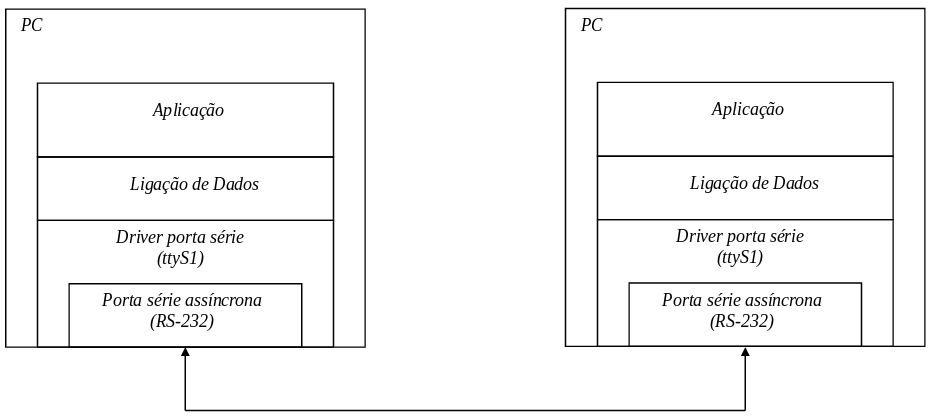
\includegraphics[width=1\textwidth]{Architecture.png}
	\caption{Program Architecture}
	\label{Image: Program Architecture}
\end{figure}

\section{Code Structure}
The application layer is implemented in the files ApplicationLayer.c and ApplicationLayer.h. As suggested in the laboratory guide, we used a struct to store this layer data.

\begin{lstlisting}
struct applicationLayer {
    int fd;
    int status; //Connection mode, 0 - Receiver, 1 - Transmitter
    unsigned int messageSize;
    char* fileName;
};
\end{lstlisting}

The functions of the application layer are:

\begin{lstlisting}
int writeControlPackage(int control, char* fileName, char * fileSize);
int initializeApplicationLayer(char* port, unsigned int messageSize, int retries, int timeout, char* fileName, int status);
int send();
int receive();
\end{lstlisting}

The link layer is implemented in the files LinkLayer.c and LinkLayer.h. Again, as suggest in the laboratory guide, we used a struct to store the data of this layer. 

\begin{lstlisting}
struct linkLayer {
    char port[20];
    unsigned int sequenceNumber;
    unsigned int timeout;
    unsigned int triesMAX;
};
\end{lstlisting}

The functions of the link layer are:

\begin{lstlisting}
void handleAlarm();
int sendMessage(int fd, char* message);
int receiveMessage(int fd, char* message);
int initializeLinkLayer(int fd, char * port, int triesMAX, int timeout);
int llopen(int fd, int connectionMode);
int llwrite(int fd, char* buffer, unsigned int length);
int llread(int fd, char* buffer);
int llclose(int fd, int mode);
unsigned int dataStuffing(char* buffer, unsigned int frameSize);
unsigned int dataDestuffing(char* buffer, unsigned int frameSize);
char findBCC2(char* data, unsigned int size);
\end{lstlisting}

The main function is in the Lab1.c file, where we store the arguments passed by the user and initialize the application layer.

\section{Use Cases}

The application has many use cases. The function llopen is used to establish the connection and the function llclose is used to close the connection. When the program is executed as transmitter, we use the function send to open the file and create the initial buffer (send) which is send by the function llwrite. When the program is executed as receiver, buffers are read through the function llread. The destination file is open so data can be written there with the function receive.

\section{Link Layer Protocol}

This protocol main objective is to organize the file information. However, opposite to the supervision frames, frames used in this protocol send information about the file. In the following code, we can see that all frames have 6 common fields: FLAG (frame[0] and frame[5 + length]), sequence bit (frame[2]), it can be 0 or 1, verification bit (frame[3]), address field (frame[1]), BCC control field (frame[4 + length]).

%\begin{figure}[h!]
	%\centering
	%\includegraphics[width=0.5\textwidth]{boardinit.jpg}
	%\caption{Initial board set up}
	%\label{Image: Initial board set up}
%\end{figure}

We also have the following function to find our BCC control field.

%\begin{figure}[h!]
	%\centering
	%\includegraphics[width=0.5\textwidth]{boardinit.jpg}
	%\caption{Initial board set up}
	%\label{Image: Initial board set up}
%\end{figure}

Our implementation includes a timeout, that is used when the connection is lost. Timeout is a value in seconds, at the end of that time, if the connection is not established the program finish. We also have a variable that says us how many tries can the program do to resend packages. If timeout didn't finished and we have already finished all tries of resending, the program finishes without timeout reach the end.

%\begin{figure}[h!]
	%\centering
	%\includegraphics[width=0.5\textwidth]{boardinit.jpg}
	%\caption{Initial board set up}
	%\label{Image: Initial board set up}
%\end{figure}

\section{Application Protocol}

The application layer contains all the higher-lever protocols. Particularly, this layer opens the port, transfers a file (sending it if it is the transmitter or receiving it if it is the receiver) and closes the port. More specifically, the application layer is responsible for the control packages (start and end) and for the data packages. In the function initializeApplicationLayer (function called in main), the port is opened, the Link Layer is initialized, it then calls send or receive function and closes the port.

In send function, after the connection is established through Link Layer, the Control Package is written and sent as START package. If no errors occur, the data packages (parts of the file that is being transferred) starts being sent. At the end, the Control Package is written and sent as END package and the connection is finished through Link Layer.

In receive function, after the connection is established through Link Layer, the Control Package is received as START package. If no errors occur, the data packages (parts of the file that is being transferred) starts being received and the file is built. At the end, the Control Package is received as END package and the connection is finished through Link Layer.

\section{Validation}

While the implementation was being done, a lot of tests were done to the program, such as, reception capacity, “pinguim.gif” image sending process. We tested with normal conditions, and after we also tested in case of losing and returning connection. In both situations we had the expected response, overcoming duplicated files and
interruptions in sending packages. Receiving “pinguim.gif” image on the receiver computer was done with success.

\section{Valuing Elements}

This program allows the user to choose the maximum size of the data packages that are going to be sent, how many times the program tries to resend packages in case of error, and even the time it waits to retry it. If any error (through BCC) is detected in a frame and it is a frame that has not been sent before, the receiver send a REJ (reject message) so it can be sent again. The program also checks the size of the file received and compares it to the size of the file sent. If any error that disables the file to be transferred entire and correctly occurs, the program is finished and error is reported to the user.

\section{Conclusion}

\end{document}
